\section{Evaluation}

\subsection{Evaluation of the hardware}

There are a few issues on the board, which have been found and fixed so far.

\textbf{Issue 1:}

The first issue is that no voltage was provided to the core of the microcontroller. This is, because
the internal voltage regulator of this package is not connected to the core. This must be done 
externally. To fix this, a switched-mode power supply was added to the board, which outputs 1\,V
for the core.

\textbf{Issue 2:}

The output voltage of the extra added power supply is noisy, which led to connection errors with the debugger.
In order to fix this, extra capacitors were added to the supply of the core.

\textbf{Issue 3:}

The input of the op-amp needs an DC-offset voltage as it has only single-supply. The offset voltage led
to DC-coupling on the input port. To fix this, a decoupling capacitor was added between the input and the op-amp.

\textbf{Current status:}

It is possible to load firmware onto the microcontroller. Also, there is the ability to sample audio data,
process it and playback the signal to the output.

A picture of the \ac{PCB} with all modifications and a potentiometer connected is shown in the appendix in \autoref{fig:pcb}.

\subsection{Evaluation of the filters}

In order to validate that the implemented filters do in fact emulate a Wah-Wah-effect,
the frequency response is measured. Additionally, the filters are subjected to a hearing test.

All these tests were done on the own build \ac{PCB}.

\subsubsection{Measurement of the \ac{FIR}- and Biquad-filters}

Firstly the \ac{FIR}-implementation is evaluated.

To measure the frequency response, an oscilloscope with a signal generator is used. Therefore a sweep
from 50\,Hz to 10\,kHz is applied to the input and a \ac{FFT} of the output is calculated. The result
of the filter at the center frequency of 460\,Hz and 2242\,Hz is shown in \autoref{fig:measure-fir}.
On channel 1 (yellow signal) is the output and on channel 2 (blue signal) the input signal. The \ac{FFT}
result is shown in purple.

\begin{figure}[!h]
    \centering
    \begin{subfigure}[c]{0.49\textwidth}
        \centering
        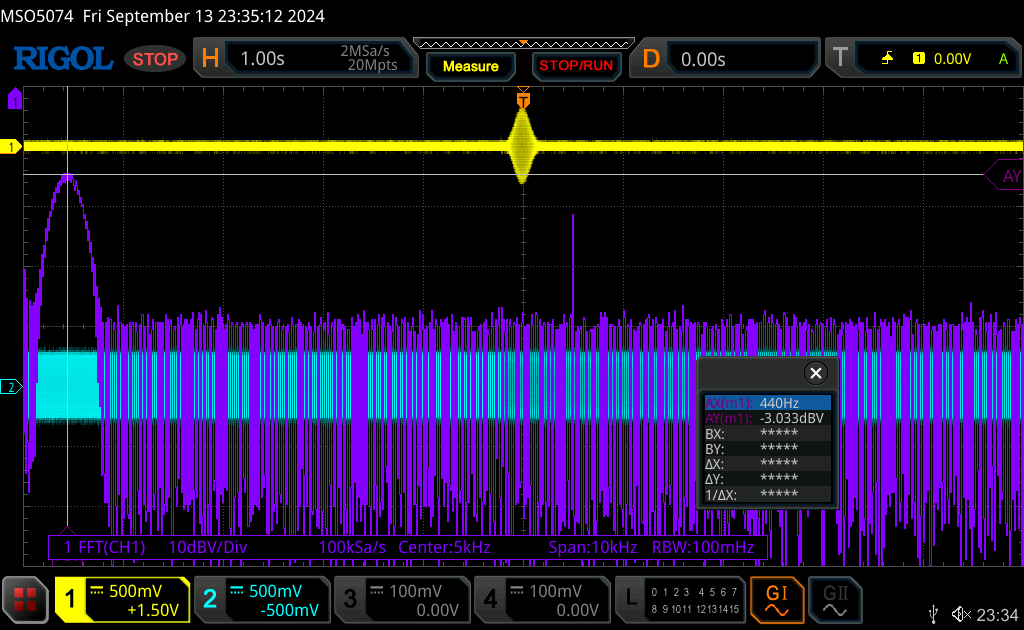
\includegraphics[width=\textwidth]{img/fir_measure_460_hamming.png}
    \end{subfigure}
    \begin{subfigure}[c]{0.49\textwidth}
        \centering
        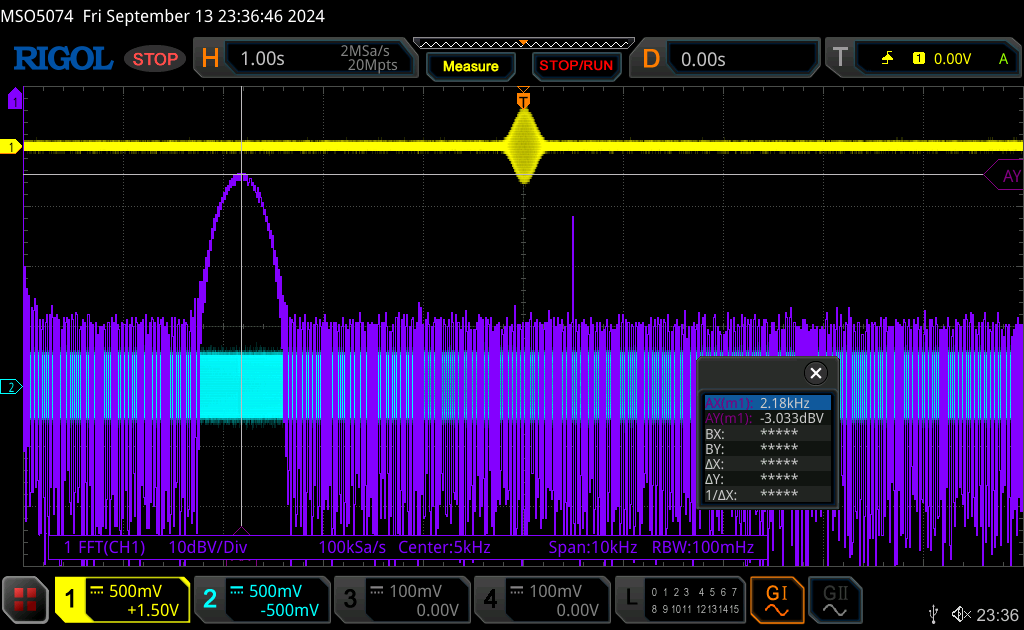
\includegraphics[width=\textwidth]{img/fir_measure_2242_hamming.png}
    \end{subfigure}
    \caption{Measurement of the \ac{FIR}-implementation using Hamming window}
    \label{fig:measure-fir}
\end{figure}

The shape of the filter are as expected in comparison to the simulation (\autoref{fig:fir-sim-hamming}).
But it has to be mentioned that the center frequencies of the filters are not exactly on the desired
frequencies. At the lowest center frequency there is a frequency shift of -20\,Hz and at the highest
-62\,Hz.

Secondly, the biquad filters are measured. The results at 460\,Hz and 2,3\,kHz center frequency are show in
\autoref{fig:measure-iir}.

\begin{figure}[!h]
    \centering
    \begin{subfigure}[c]{0.49\textwidth}
        \centering
        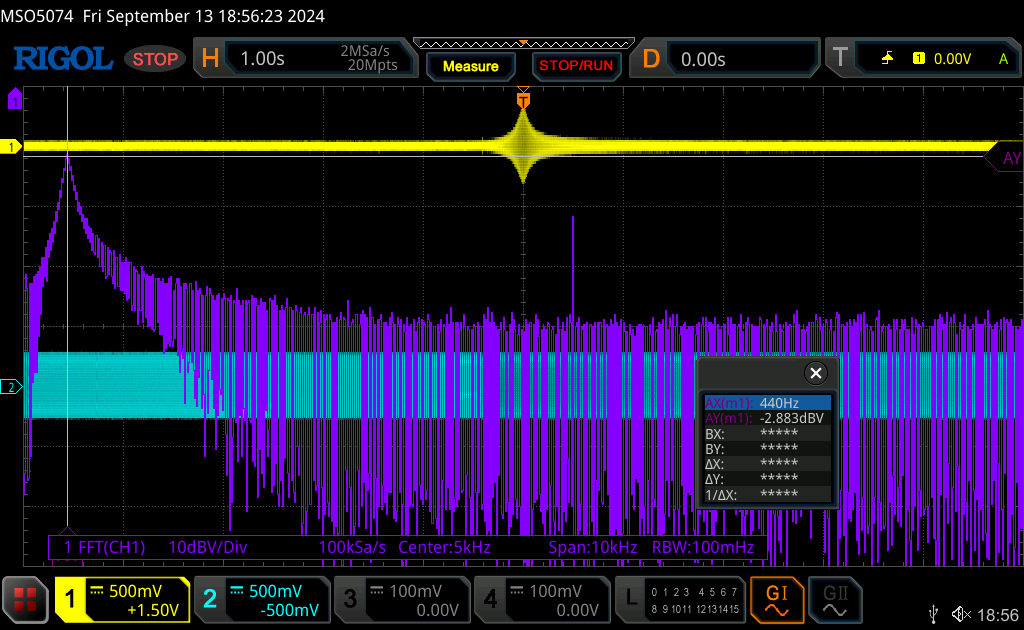
\includegraphics[width=\textwidth]{img/iir_measure_460.png}
    \end{subfigure}
    \begin{subfigure}[c]{0.49\textwidth}
        \centering
        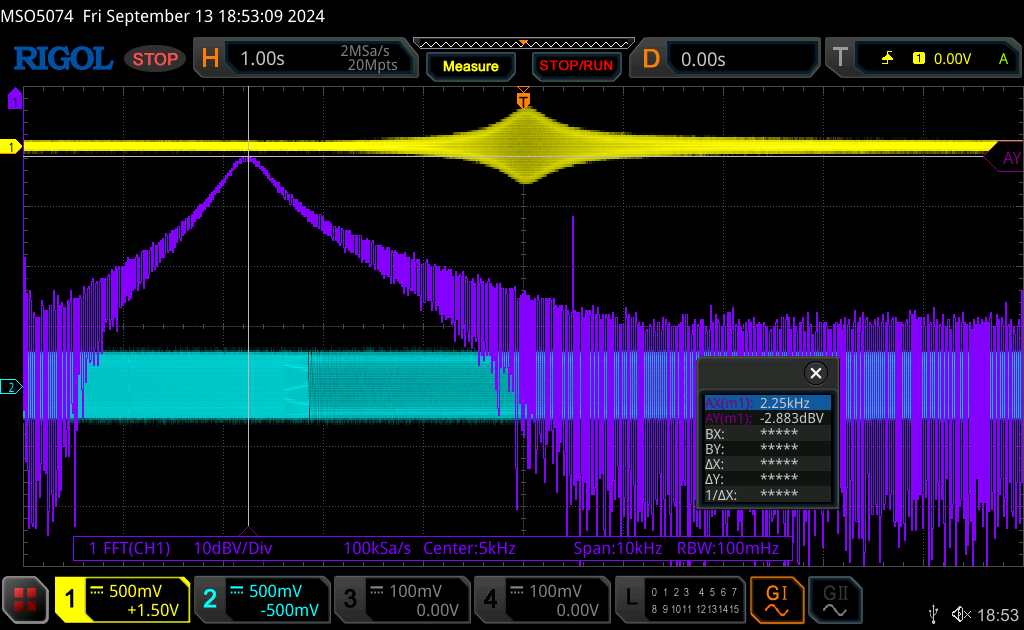
\includegraphics[width=\textwidth]{img/iir_measure_2300.png}
    \end{subfigure}
    \caption{Measurement of the biquad-implementation}
    \label{fig:measure-iir}
\end{figure}

Also, this result is as expected except the frequency shift. There is also a frequency shift of -20\,Hz at
the lowest frequency and -75\,Hz at the highest frequency.

Probably this is the result of a slight difference of the desired and the real sampling rate. This can be
fixed by adjusting the sampling frequency when generating the coefficients.

In order to measure the latency of the system, a step was given to the input and the time difference to
the step response is measured. This is shown in \autoref{fig:measure-step-response}.

\begin{figure}[!h]
    \centering
    \begin{subfigure}[c]{0.49\textwidth}
        \centering
        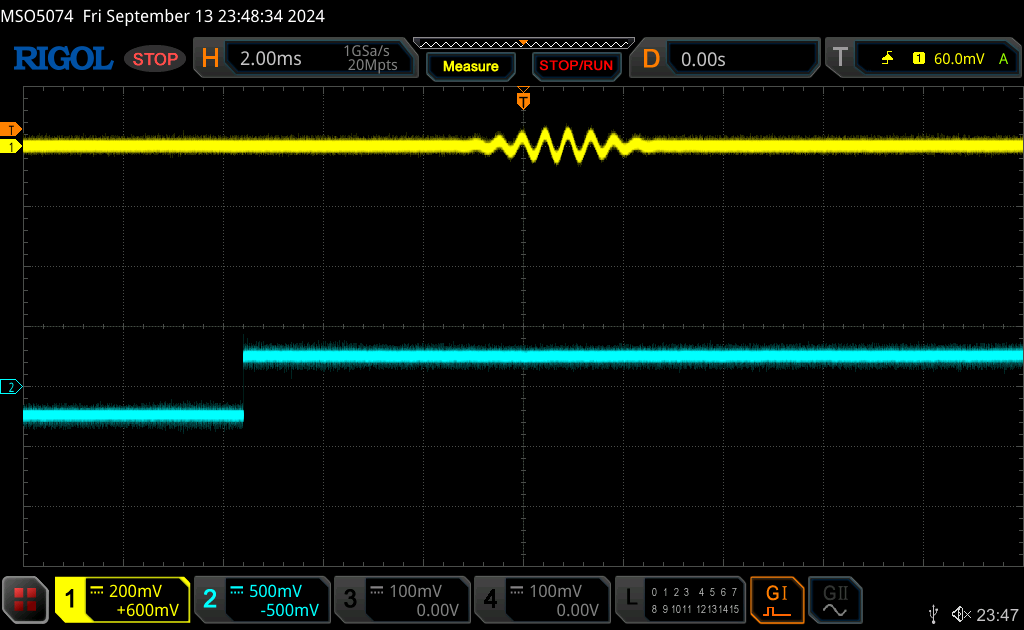
\includegraphics[width=\textwidth]{img/step_response_2242_fir_hamming.png}
    \end{subfigure}
    \begin{subfigure}[c]{0.49\textwidth}
        \centering
        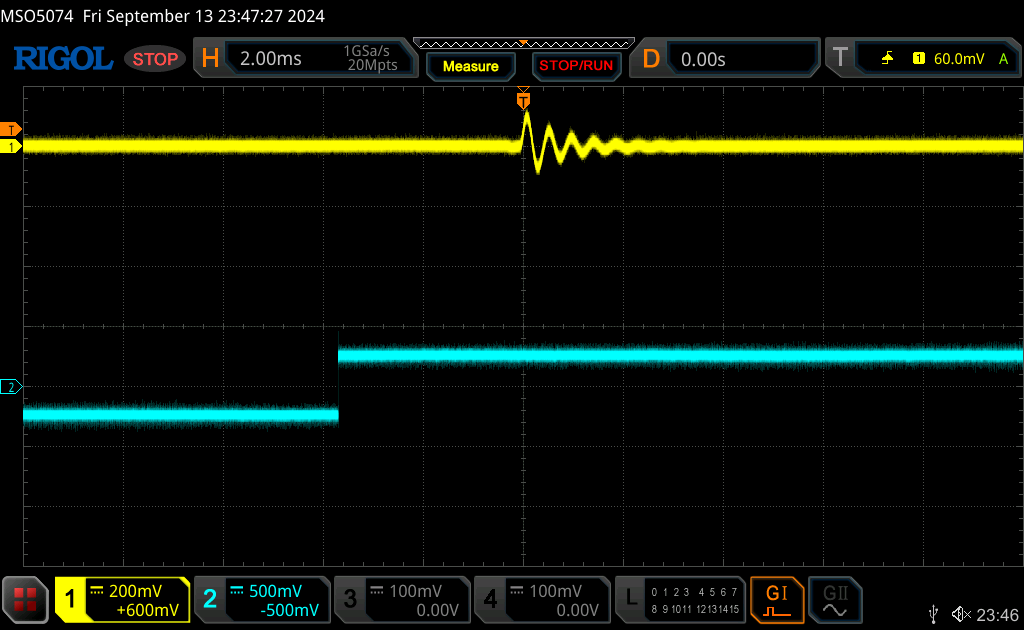
\includegraphics[width=\textwidth]{img/step_response_2300_iir.png}
    \end{subfigure}
    \caption{Measurement of the step response of the \ac{FIR}- and Biquad filters}
    \label{fig:measure-step-response}
\end{figure}

As it can be seen, the latency of the \ac{FIR}-filter with 4,8\,ms is higher than the Biquad-implementation
with about 3,6\,ms. Both filters fulfill the requirement of a maximum latency of 5\,ms.

\subsubsection{Hearing-tests of the implemented filters}

The goal is to compare the \ac{FIR}- with the Biquad implementation related to its audible properties.
Because this is highly subjective, this is not an absolute or general result.

At the highest frequency ($\sim$2,2\,kHz) there is a noticeable difference. The \ac{FIR}-implementation seems
to be less broadband. This was tested by playing the same riff on the guitar, which includes notes on the low E-string and
the G-, B- and high E-string. The notes on the low E-string seemed to be more attenuated than in the
Biquad-implementation. This is reasonable as this is the behaviour the frequency response of the \ac{FIR}-filters
looks like.

If the filter at 440\,Hz is applied, the difference is not as noticeable as at higher center frequencies.

The final test is the evaluation by adjusting the center frequency at runtime. Therefore a footpedal in which
a potentiometer is built in, is connected to one of the analog input pins.

For the \ac{FIR}-implementation
there is some cracking noise on the output signal. This could be caused by loading the coefficients from a lookup table
to the filter which take some time to be processed. In this time, some samples can get lost.
This could be improved by for example loading the coefficients asynchronously.

The \ac{IIR}-implementation works without cracking noise, as the amount of coefficients is much smaller, although
they are being computed every process step.

In general the sound with the recursive filter sounds more \frqq natural\flqq{} than
with the \ac{FIR}-filter used.

Also the noticable latency is evaluated. A significant delay was recognized with a buffer size of 2048 samples.
